\newtoggle{withbonus} \toggletrue{withbonus} % set true to show bonus points in grade table

% setting underlying course name (Grundlagenfach Mathematik, §-Unterricht, \ldots)
\newcommand{\mycourse}{Grundlagenfach Informatik}
% name of the class
\newcommand{\myclass}{3. Klassen}
% set date
\newcommand{\mydate}{13. September 2024}

\title{\textbf{Hardware}}
\author{Thomas Graf\\
\mycourse, \myclass}
\date{\mydate}
\maketitle
\thispagestyle{headandfoot}		
\clearpage

\begin{questions}

\question[2]

Gib die Wertetabelle an, die durch folgende Schaltung erzeugt wird:
\begin{figure}[H]
    \centering
    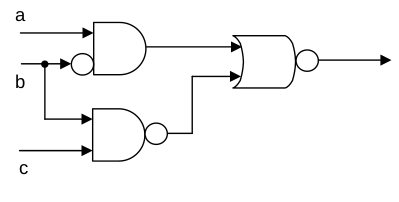
\includegraphics[scale=0.6]{EF/Exams/aufgabe01.png}
\end{figure}
Hinweis: Der \enquote{Kreis} ist eine Kurzschreibweise für einen Inverter (Negation) \begin{tikzpicture}\node[not gate US, draw] (Not1) {};\end{tikzpicture}. Bezeichne das Outputsignal in deiner Wahrheitstabelle entweder mit \textit{d} oder mit \textit{Out}.

\begin{solution}
    Die gesuchte Wahrheitstabelle (wir bezeichnen das Outputsignal mit \textit{d}) lautet:
\begin{figure}[H]
    \centering
    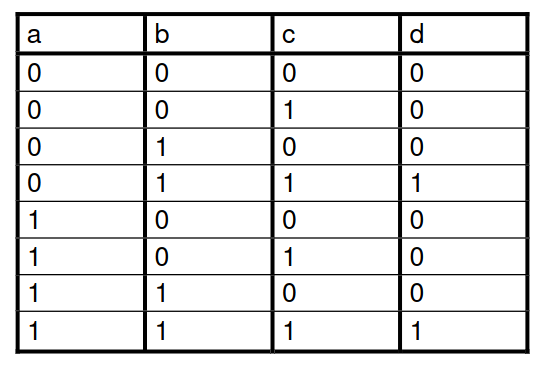
\includegraphics[scale=0.6]{EF/Exams/sol_aufgabe01.png}
\end{figure}
\end{solution}
\clearpage
\question
Betrachte die nachfolgende Abbildung.
\begin{figure}[H]
    \centering
    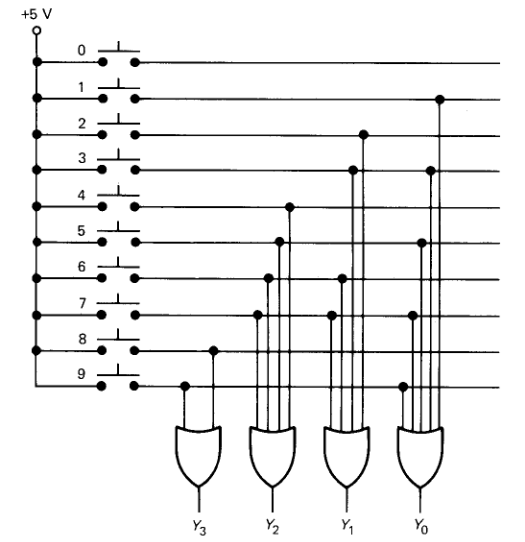
\includegraphics[scale=0.6]{EF/Exams/aufgabe02.png}
\end{figure}
Der Output dieser Schaltung ist das binäre Wort $Y_3Y_2Y_1Y_0$ der Länge 4. Bei den Ziffern 0 bis 9 ist jeweils ein Drückschalter (push-button switch) wie bei einem Taschenrechner angebracht. Wir gehen hier davon aus, dass zu jeder Zeit höchstens einer der Drückschalter gedrückt (geschlossen) wird!
\begin{parts}
    \part[1] Wie lautet das Outputwort, wenn genau der Drückschalter bei Ziffer 3 (und kein anderer) gedrückt (geschlossen) wird?
    \begin{solution}
    Das Outputwort lautet dann $0011$.
    \end{solution}
    \part[1] Wie lautet das Outputwort, wenn genau der Drückschalter bei Ziffer 5 (und kein anderer) gedrückt (geschlossen) wird?
    \begin{solution}
    Das Outputwort lautet dann $0101$.
    \end{solution}
    \part[2] Was tut diese Schaltung? Wieso / warum könnte eine solche Schaltung z.B. in einem Taschenrechner eingesetzt werden?
    \begin{solution}
    Eine solche Schaltung wird \textit{decimal-to-binary encoder} genannt. Das Drücken des Schalters gehörend zu Ziffer $n$ erzeugt ein Outputwort, welches genau der binären Darstellung der Ziffer $n$ entspricht. So wird z.B. beim Drücken vom Schalter bei Ziffer 9 das Outputwort $1001$ angenommen --- dies ist die binäre Darstellung der 9. In einem Taschenrechner kann dadurch dezimaler Userinput in das Binärsystem (zur weiteren Verarbeitung im binär arbeitenden Taschenrechner) umgewandelt werden (encoding).
    \end{solution}
\end{parts}
\droptotalpoints
\end{questions}
